\subsection{Prog-poly: Jogo de tabuleiro baseado no monopoly para ajudar nos estudos de linguagem de programação e engenharia de software}

Durante o trabalho de pesquisa de mestrado \textit{Prog-poly}, foi desenvolvido um jogo de tabuleiro com o intuito de facilitar e auxiliar a aprendizagem de temas como linguagem de programação e engenharia de software. Este jogo foi baseado na mecânica do clássico jogo de tabuleiro Monopoly, onde cada jogador deve comprar propriedades no tabuleiro. Entretanto, este jogo se diferencia pois para ter a oportunidade de comprar a propriedade, o jogador deve responder de forma correta perguntas a respeito de \emph{ILPC} (Introdução Linguagem de Programação C) e, somente se acertar, poderá adquirir a propriedade, caso possua dinheiro suficiente. Ganha o jogador que possuir a maior quantidade de dinheiro e propriedades.

Este Jogo se caracteriza por ser um jogo com uma abordagem de ensino explicita, pois se trata de um \emph{quiz}. \cite{nascimento2022prog}

\begin{figure}[H]
	\centering
	\caption{Captura de tela do tabuleiro de Prog-poly}
	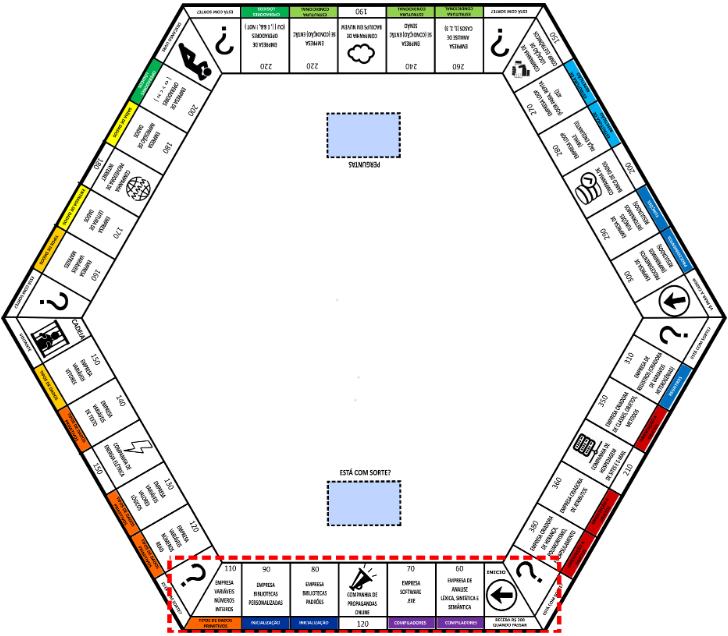
\includegraphics[width=0.8\textwidth]{images/prog-poly.png}
	\legend{Fonte: \cite{nascimento2022prog}}
	\label{fig:prog_poly}
\end{figure}

